\documentclass[12pt]{article}
\usepackage{lscape, xcolor}
\usepackage{verbatim}
\usepackage{amsmath,amsthm,amssymb}
\usepackage{colonequals,color,multirow}
\usepackage{enumerate}
\usepackage[sc]{mathpazo} % Use the Palatino font
\usepackage[T1]{fontenc} % Use 8-bit encoding that has 256 glyphs
\usepackage{times}	
% \usepackage{apacite}
\usepackage[authoryear]{natbib}
\usepackage[demo]{graphicx}
\usepackage{subcaption}
\usepackage{lscape, xcolor}
\usepackage{verbatim}
\usepackage{amsmath,amsthm,amssymb}
\usepackage[sc]{mathpazo} % Use the Palatino font
\usepackage[T1]{fontenc} % Use 8-bit encoding that has 256 glyphs
\usepackage{times}	
\usepackage{booktabs}
\usepackage{ caption, float}
\usepackage{enumitem}
\usepackage[left=1in, right=1in, top=1in, bottom=1in]{geometry}
\usepackage{blindtext}
\usepackage{titlesec}
\usepackage{array}
\usepackage{graphicx}
%\graphicspath{/home/evo/4m_final_project}
\setcounter{secnumdepth}{4}
\usepackage{caption} % For subfigures with captions
\usepackage{subcaption} % For subfigures with captions
\captionsetup[subfigure]{labelformat=empty} % Removes the (a), (b) labels
\usepackage{hyperref}
\usepackage[authoryear]{natbib}
\usepackage{setspace}
%\onehalfspacing % Sets one-and-a-half line spacing globally
\titleformat{\paragraph}
{\normalfont\normalsize\bfseries}{\theparagraph}{1em}{}
\titlespacing*{\paragraph}
{0pt}{3.25ex plus 1ex minus .2ex}{1.5ex plus .2ex}
\renewcommand{\baselinestretch}{1.5}% Line spacing - Palatino needs more space 
\vspace{\baselineskip}
\linespread{1.5}
\setlength{\parskip}{0.5em} % Adjust spacing to 0.5em (smaller than default)




\begin{document}

\title{STATS 4M03: Multivariate Analysis\\ Final Project \\ Diabetes Dataset }

\author{Submitted to\\ Dr. Eman M.S. Alamer 
\\Department of Mathematics and Statistics
\\McMaster University\\Hamiltion, Ontario, Canada L8S 4K1}
\date {November 22, 2024}


\maketitle

 \centerline{Reported by}
 \centerline{Xinyi Chen (400326045)}
  \centerline{Tonu Xu(400370837)}
   \centerline{Rayyan Kazim(Student ID)}
    \centerline{Safi Khan (400402095)}
     \centerline{First last (Student ID)}


\newpage
%\thispagestyle{fancy} % All pages have headers and footers
\section{Introduction}
\subsection{Abstract}

\begin{indent} 

The study of diabetes is vital in understanding the progression of the disease and identifying key predictors. Throughout this paper, we perform data analysis on the diabetes dataset, primarily focusing on leveraging various statistical methods that we learned in STATS 4M03$\backslash$6M03: Multivariate Analysis. By using a variety of methods, our goal is to predict the onset of diabetes from detailed medical diagnostic measurements based on several contributing health factors --- with the aim of uncovering patterns and relationships between various clinical and lifestyle factors. Through this analysis, we hope to emphasize actionable insights for clinical decision-making and provide preventive strategies. 

\end{indent}

\subsection{The Data}

\begin{indent}

In this paper, we will study the \href{https://www.kaggle.com/datasets/hasibur013/diabetes-dataset}{Diabetes Dataset}. \cite{Kaggles}, which contains 768 rows x 9 columns. Each column represents various health diagnostic metrics for predicting diabetes and each row corresponds to a unique patient record, with features capturing key medical attributes. Table~\ref{tab:DibetesTab} showcases each of the columns in the dataset and a description of each of the columns. We will be using R \cite{Rlang} as our main computing software

\end{indent}


\begin{table}[h!]
	\centering
	\resizebox{=\textwidth}{!}{ % Resize to fit the width of the page
	\begin{tabular}{|c|c|}
		\hline
		\textbf{Column} & \textbf{Description Of Column} \\ \hline
		Pregnancies & Integer: Number of times the patient has been pregnant. \\ \hline
		Glucose & Integer: Plasma glucose concentration (mg/dL) after a 2-hour oral glucose tolerance test. \\ \hline
		BloodPressure & Integer: Diastolic blood pressure (mm Hg). \\ \hline
		SkinThickness & Integer: Triceps skinfold thickness (mm). \\ \hline
		Insulin & Integer: 2-hour serum insulin (mu U/ml). \\ \hline
		BMI  & Float: Body mass index, defined as weight in kg/(height in m)\^2. \\ \hline
		DiabetesPedigreeFunction & Float: A score indicating genetic predisposition to diabetes based on family history. \\ \hline
		Age & Integer: Age of the patient (in years). \\ \hline
		Outcome & Binary: Target variable where 1 indicates diabetes, and 0 indicates no diabetes. \\ \hline
	\end{tabular}
}
	\caption{Description of the Diabetes Dataset}
	\label{tab:DibetesTab}
\end{table}


\subsubsection{Exploratory Data Analysis (EDA)}

<<<<<<< HEAD
\begin{enumerate} 
	
	\item The diabetes dataset consists of 768 observations and 9 variables. All variables are integers, except for "BMI" and "DiabetesPedigreeFunction", which are labelled as numeric. This dataset does not consist of any N/A values or duplicated rows. 
	
	\item A summary statistics table was used to show the mean, median, minimum and maximum values of each variable, as well as quartiles. There are a lot more observations without diabetes than with diabetes. The ages listed in this dataset follow a right-skewed distribution, where majority of the individuals are aged 20-30. 
	
	\item "SkinThickness" is well correlated with "BMI" and "Insulin". "Glucose" is reasonably correlated with "Insulin", "BMI" and also "Age". "Age" is well correlated with "Pregnancies". 
	
	\item The dataset will be split into 2, where 1 will be the response variable, "Outcome". The other will consist of all the other variables, which are considered the predictor variables. All predictors should be used as they all are numeric/integer variables who are well/reasonably correlated with each other. 75 percent of the data will be used for training, whereas the rest will be used for testing. 
	
	\item For dimensionality reduction, we cannot use factor analysis since the dataset is not normally distributed. This can be confirmed by the shapiro test \cite{Rlang} and normal QQ plot \cite{Rlang}. For dimensionality reduction, we would use principal component analysis. We will use 3 principal components.\\  
	
	
	
	% \begin{figure}[h!] 
		
	% 	\centering 
		
	% 	\fbox{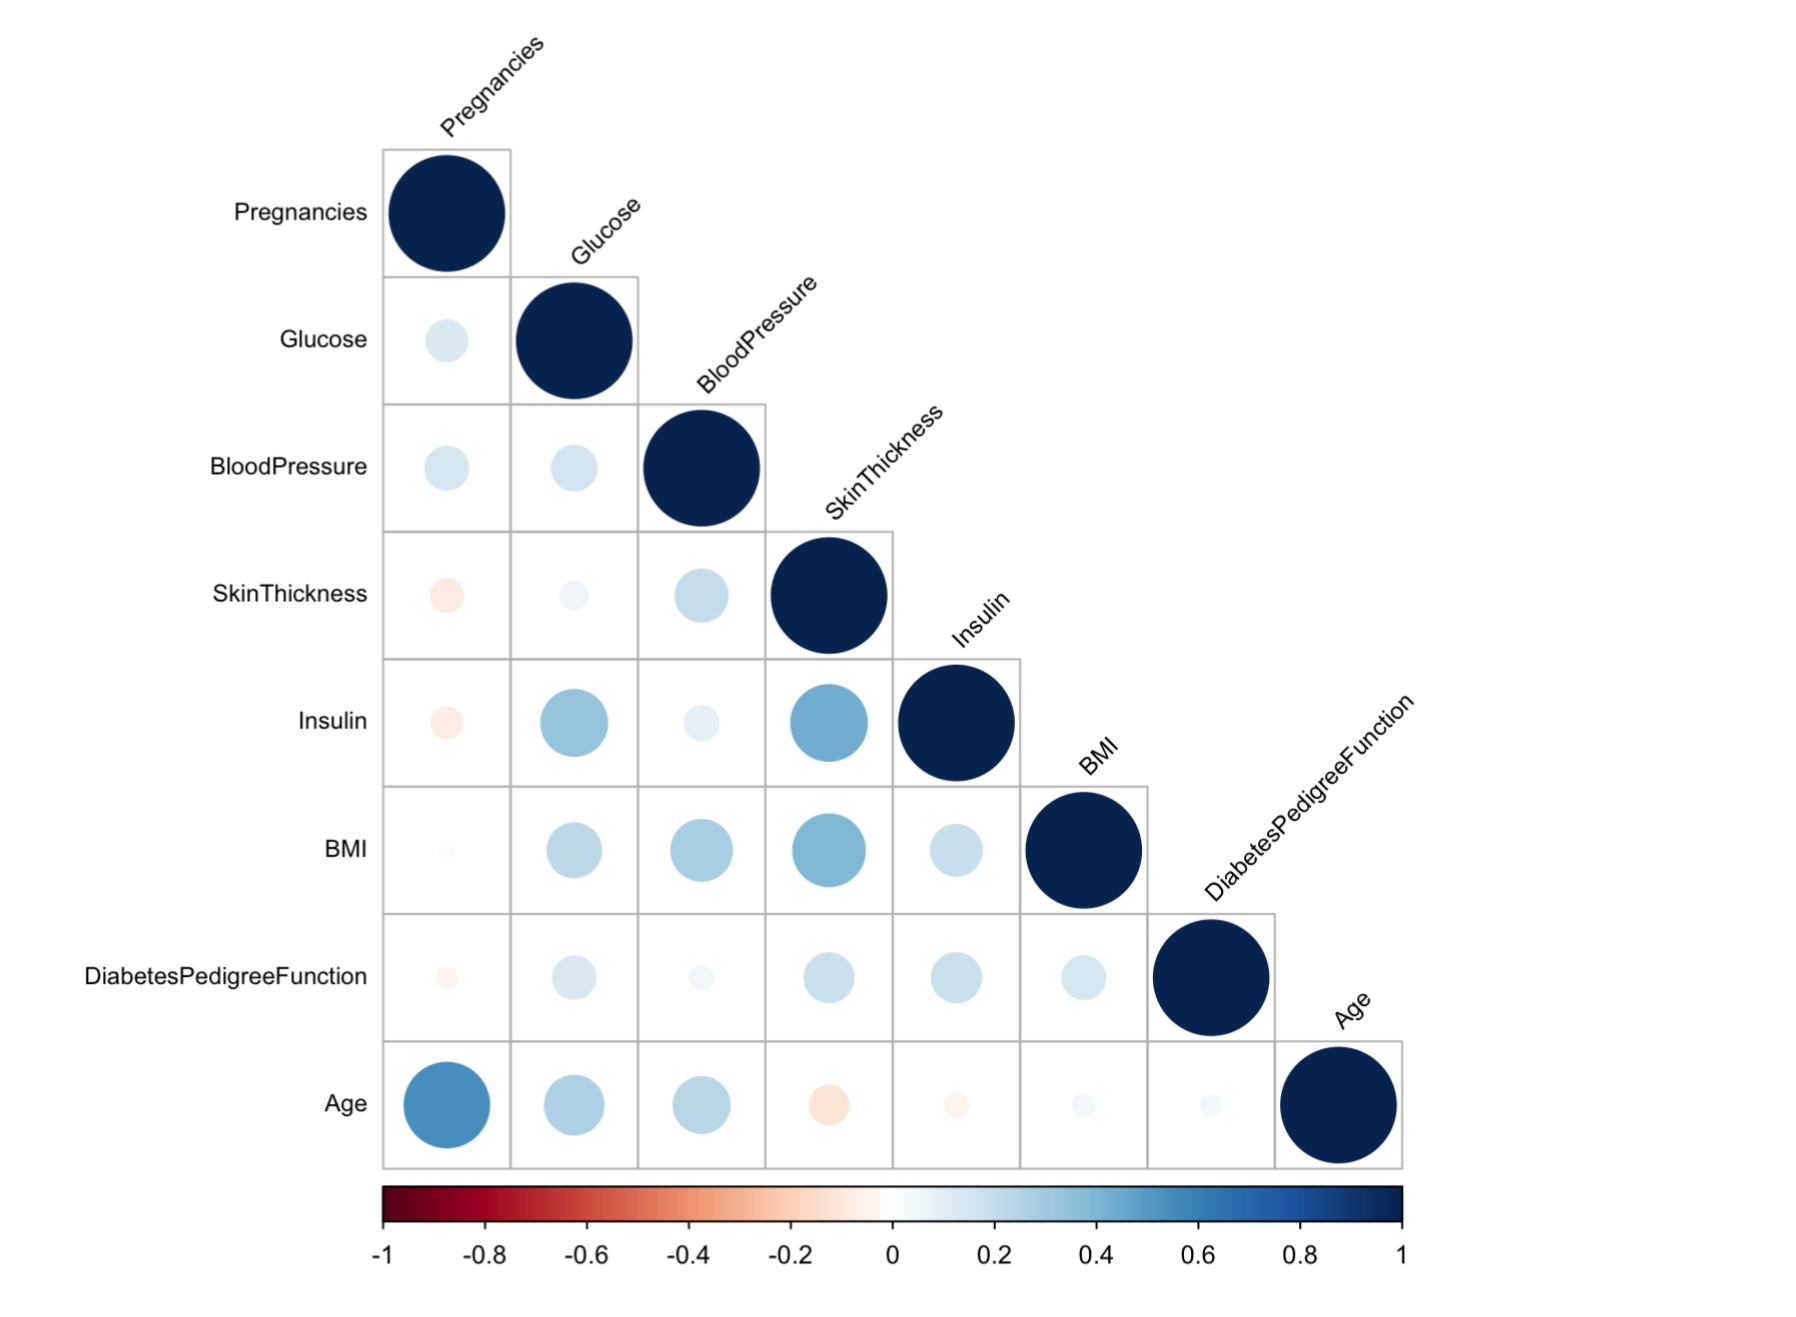
\includegraphics[width=0.62\textwidth]{correlations2.png}} 
		
	% 	\caption{Correlation Plot} 
		
	% 	\label{fig:corplot} 
		
	% \end{figure} 
	
	
	
	% \begin{figure}[h!] 
		
	% 	\centering 
		
	% 	\fbox{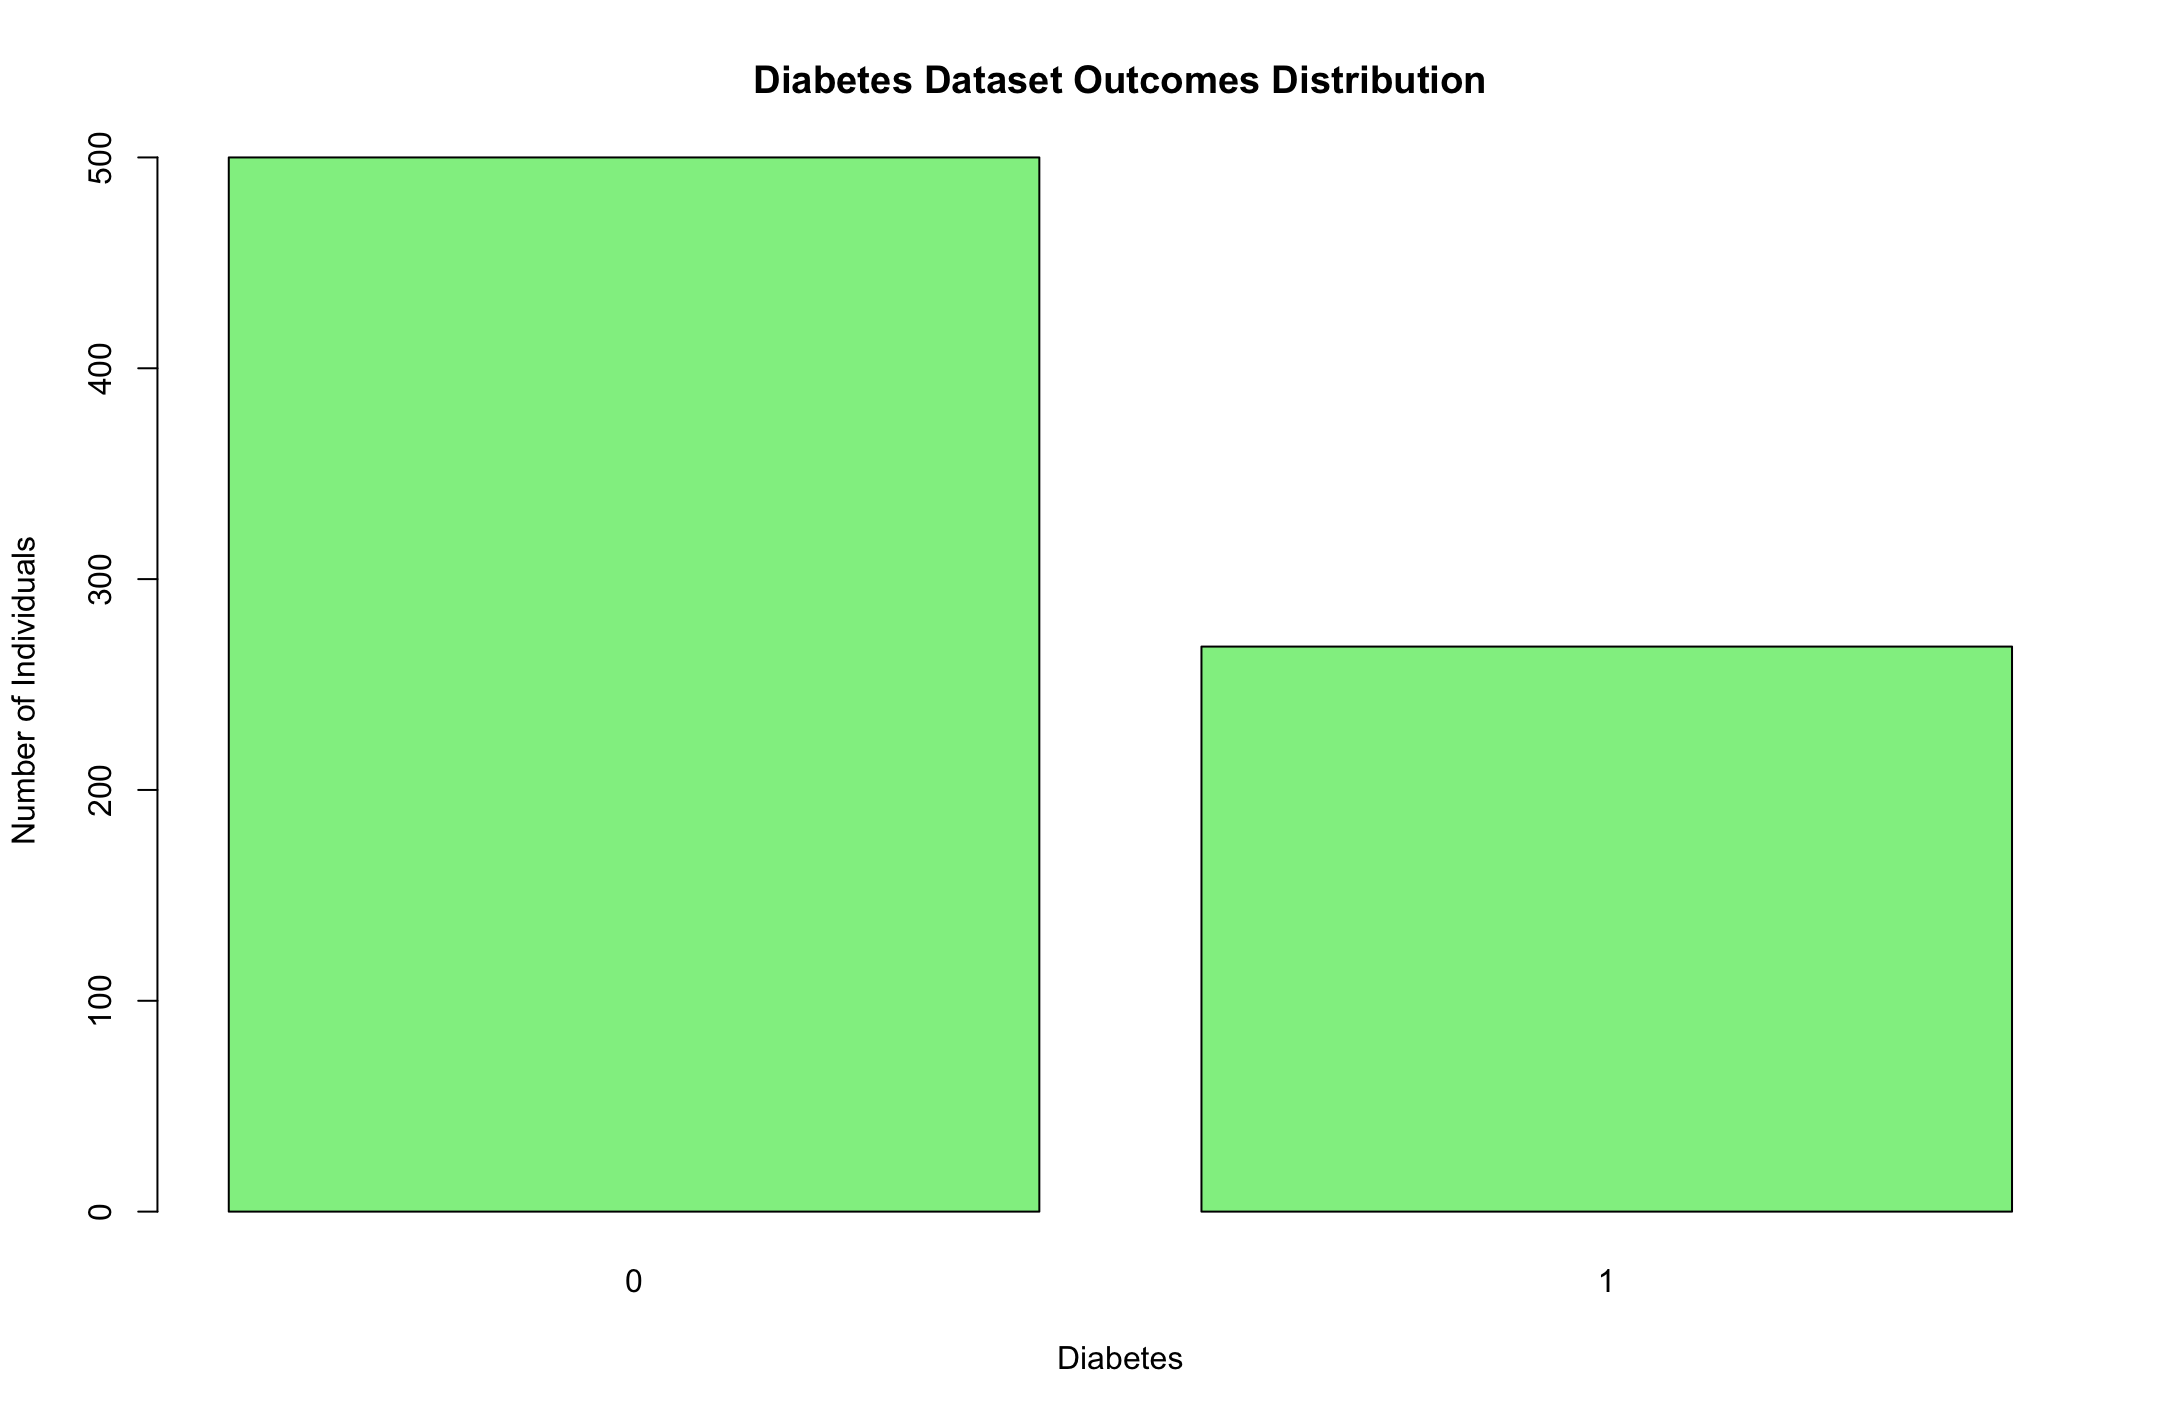
\includegraphics[width=0.62\textwidth]{outcomes.png}} 
		
	% 	\caption{Outcomes Plot} 
		
	% 	\label{fig:barplot} 
		
	% \end{figure} 
	
	
	
	% \begin{figure}[h!] 
		
	% 	\centering 
		
	% 	\fbox{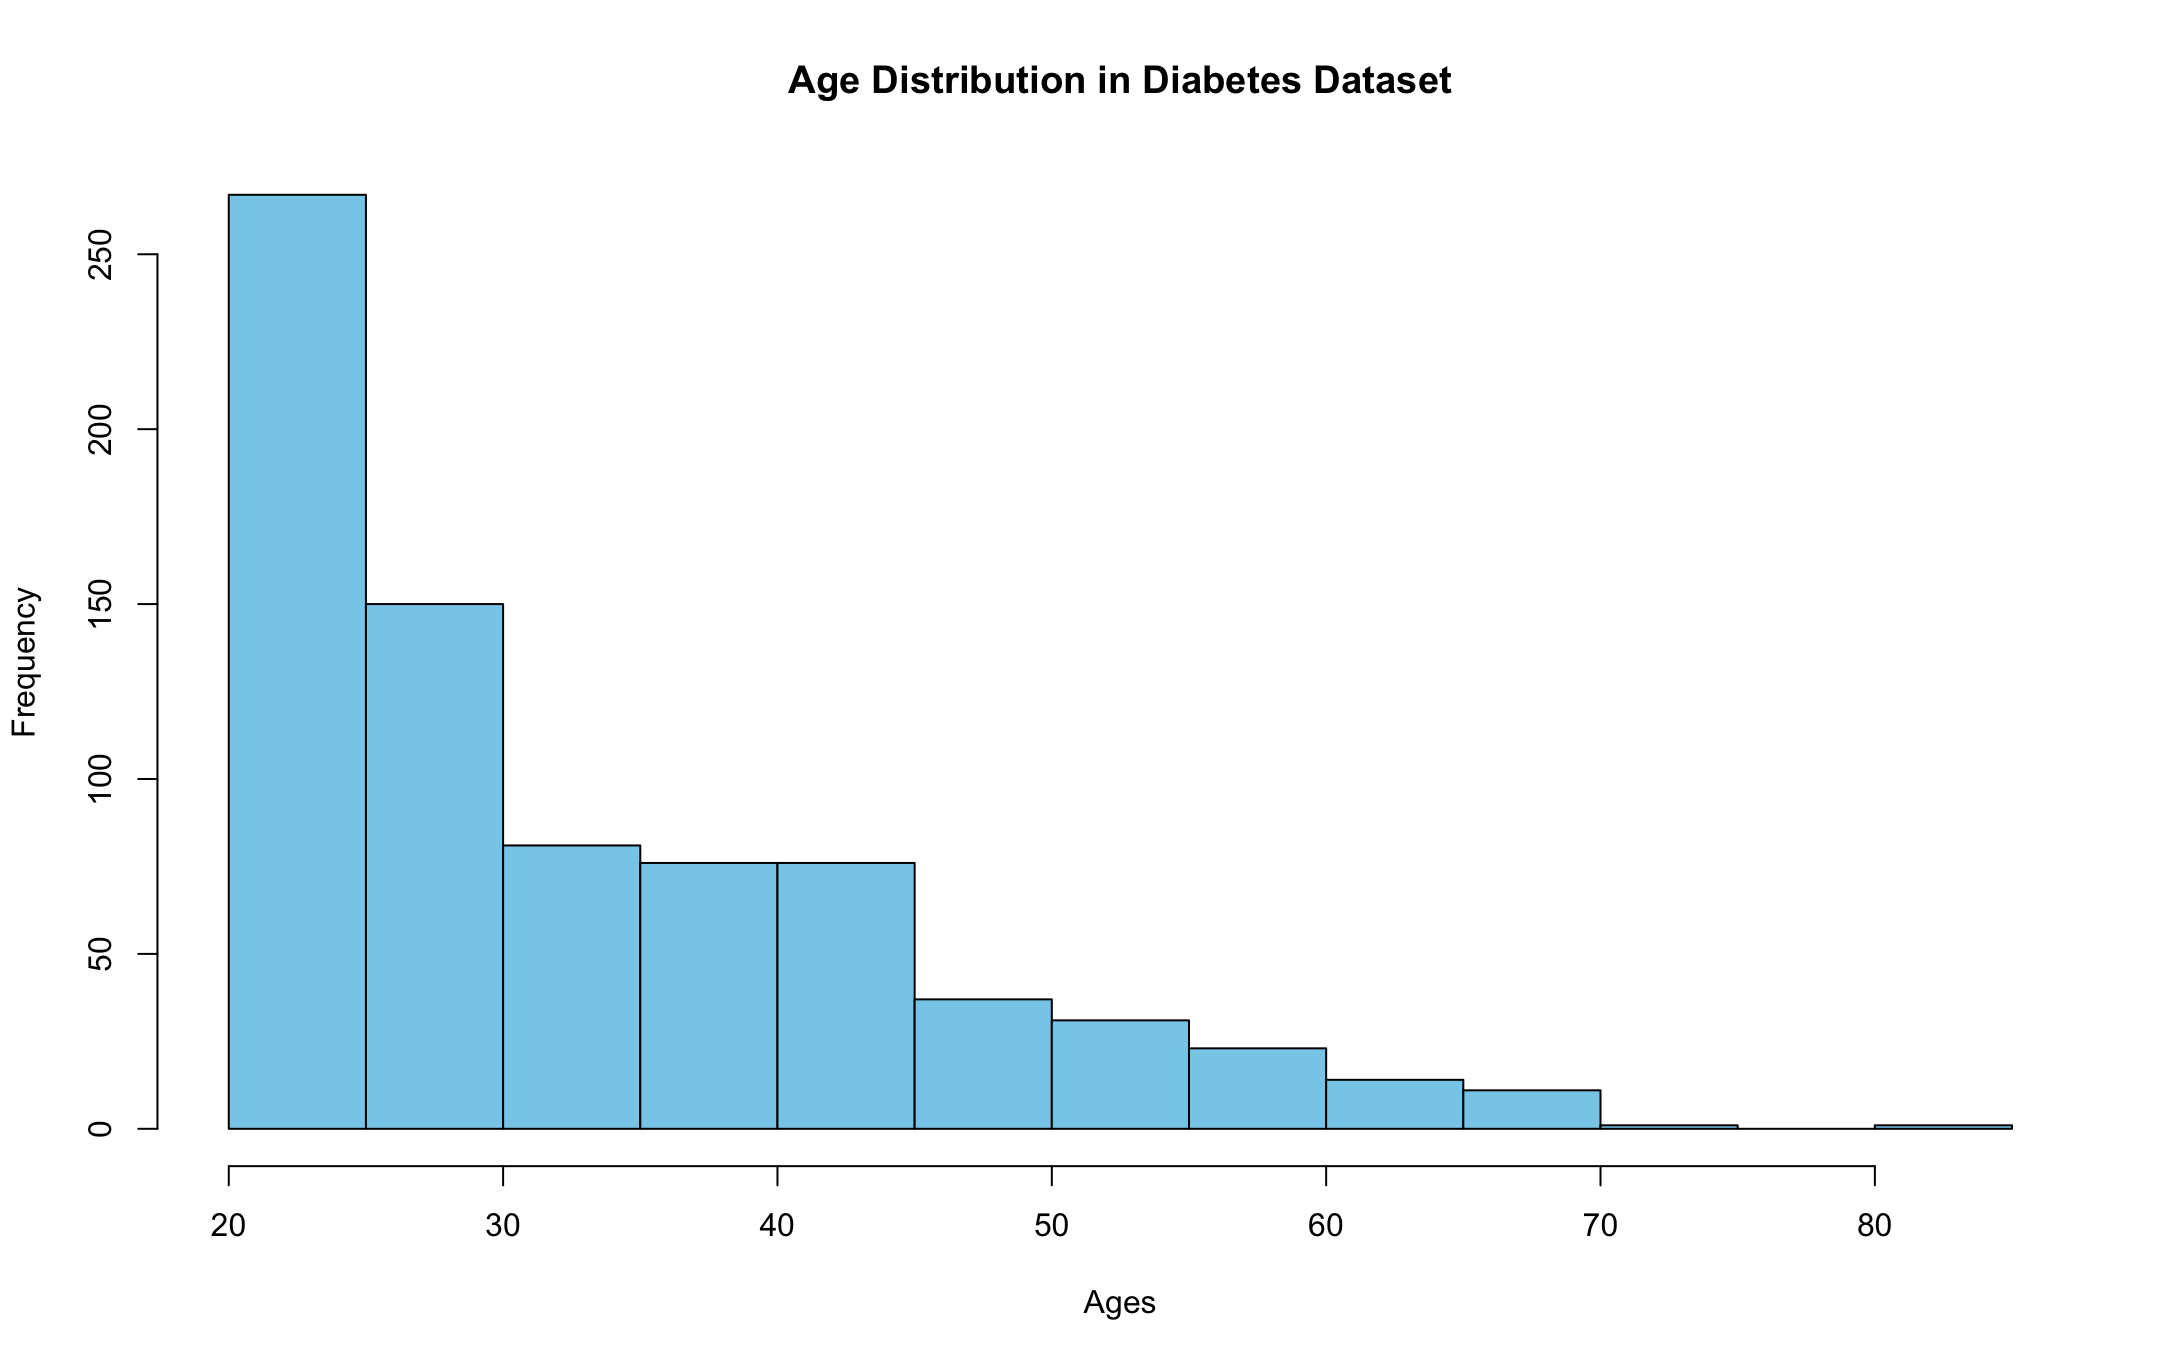
\includegraphics[width=0.62\textwidth]{ages.png}} 
		
	% 	\caption{Ages Plot} 
		
	% 	\label{fig:histplot} 
		
	% \end{figure} 
	
	
	
	% \begin{figure}[h!] 
		
	% 	\centering 
		
	% 	\fbox{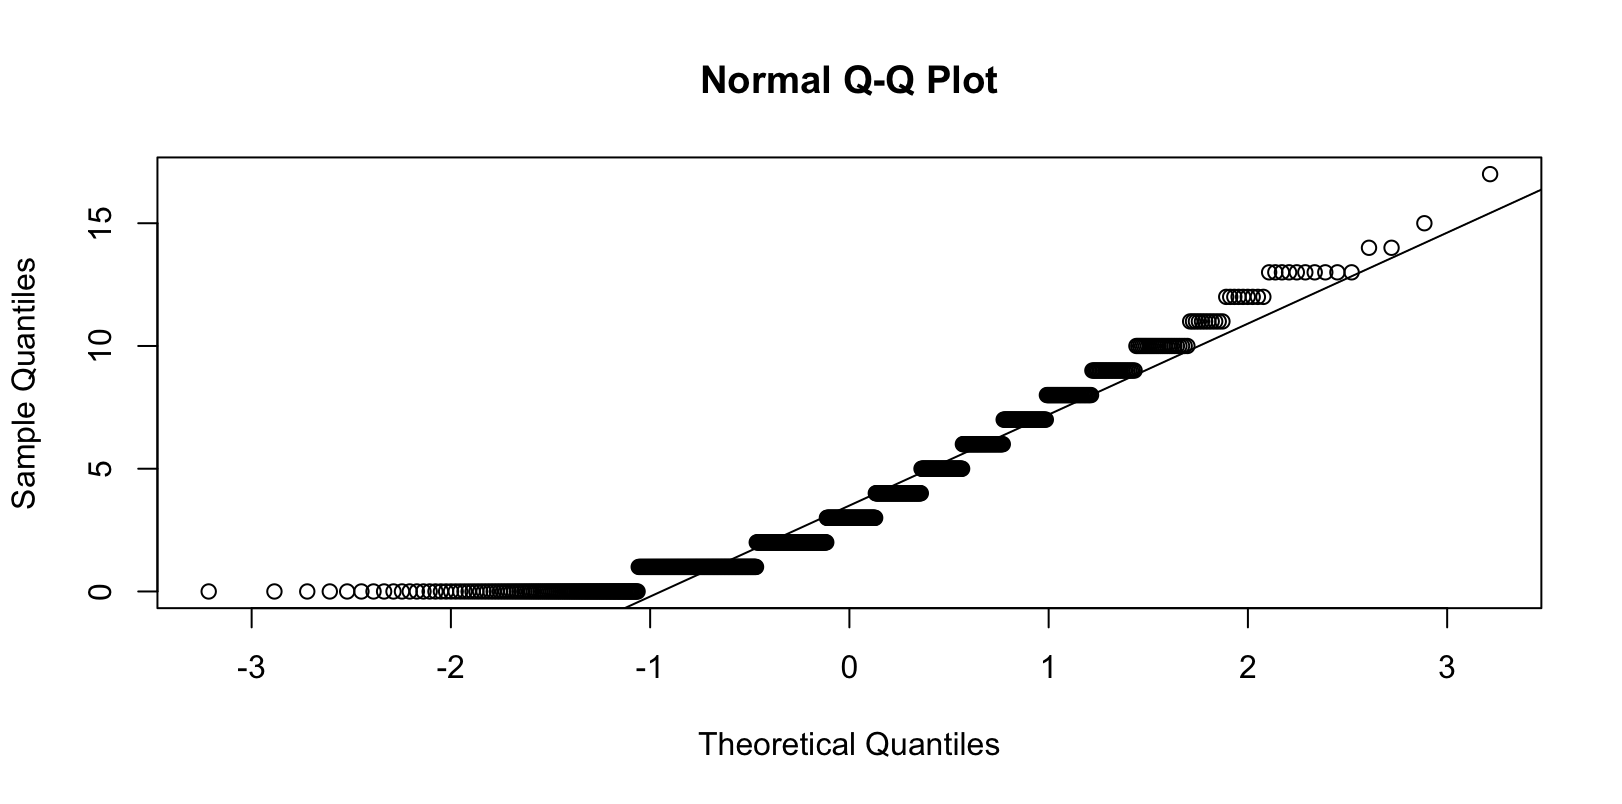
\includegraphics[width=0.62\textwidth]{normal.png}} 
		
	% 	\caption{Normality Checking Plot} 
		
	% 	\label{fig:normalplot} 
		
	% \end{figure} 
		
\end{enumerate}
 
=======
Figure~\ref{fig:outcomeplot} illustrates that there are a lot more individuals without diabetes than with diabetes. Figure~\ref{fig:ageplot} showcases that the ages listed in this dataset follow a right-skewed distribution, where majority of the individuals are aged 20-30.
>>>>>>> 19eb991fa5b0a3d3b3f1ccf045208115b78154c7

Figure~\ref{fig:corplot} illustrates the relatively high correlation between "SkinThickness," "BMI," and "Insulin." We also note that "Glucose" is reasonably correlated with "Insulin," "BMI," and "Age." Furthermore, "Age" is highly correlated with "Pregnancies."

The true label of this dataset is "Outcome," whereas the other variables are considered the predictors. Since our dataset is not that large, we determined that we should use all of the predictors as they all show reasonably high correlation with each other. 75\% of the data will be used for training, whereas the rest will be used for testing.

We cannot apply factor analysis on our dataset as it is not normally distributed. This can be confirmed by the Shapiro-Wilk test and normal QQ plot. For dimensionality reduction, we would use principal component analysis. We will use 3 principal components.

\begin{figure}[h!]
	\centering
	% First figure
	\begin{minipage}{0.48\textwidth}
		\fbox{{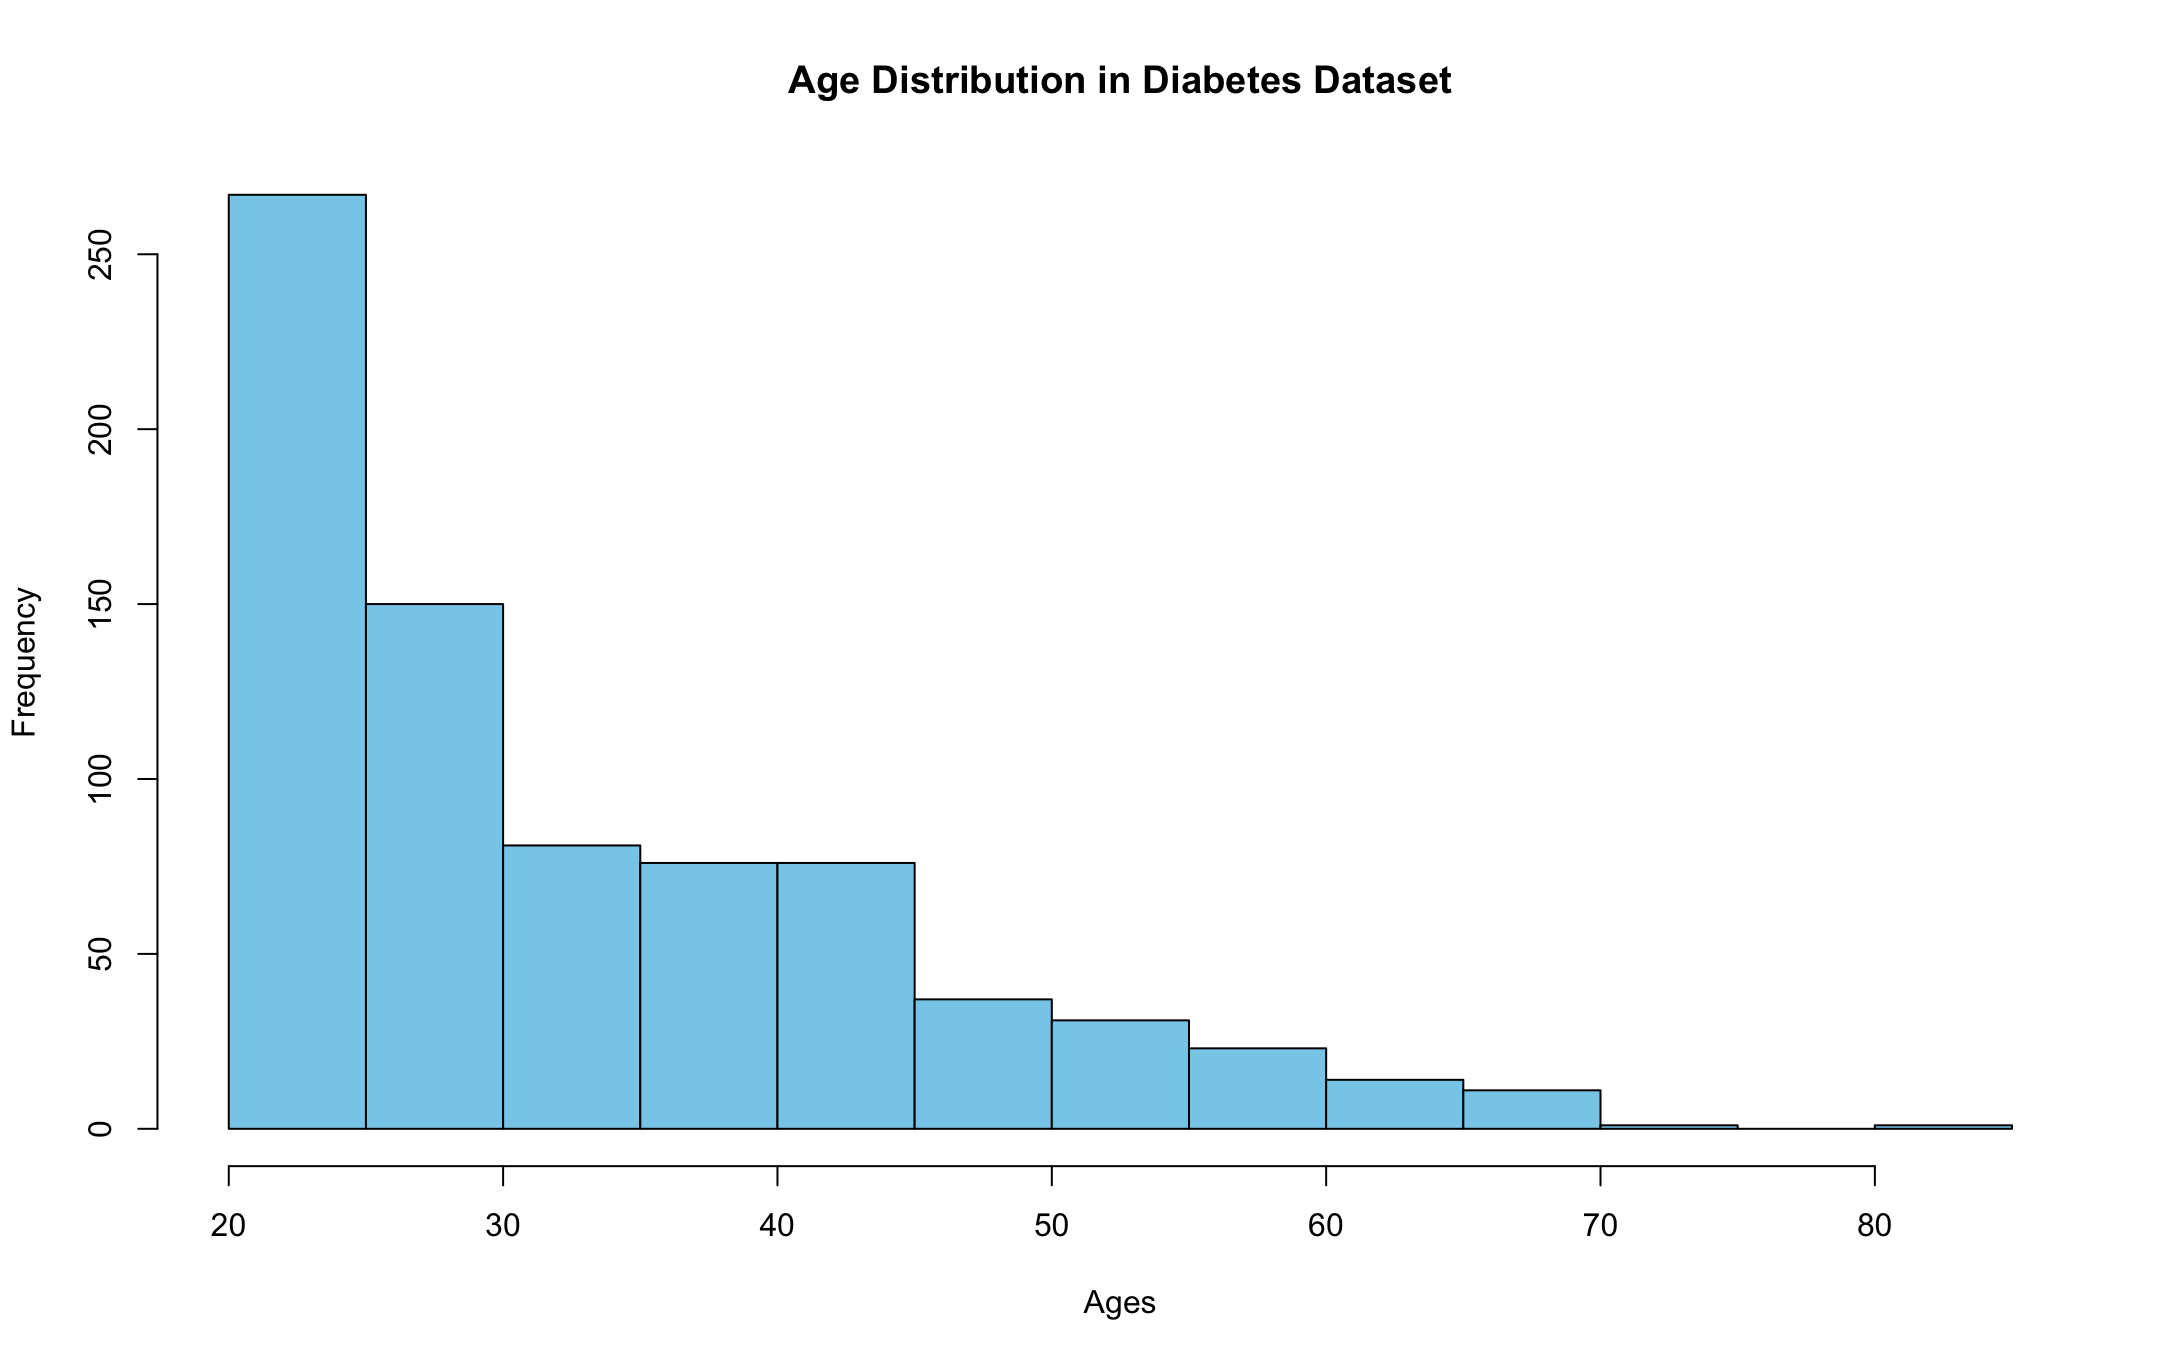
\includegraphics[width=\textwidth]{ages.png}}}
		\caption{Age Distribution of the Dataset} 
		\label{fig:ageplot}
	\end{minipage}
	\hfill % Horizontal space between figures
	% Second figure
	\centering
	\begin{minipage}{0.48\textwidth}
		\centering
		\fbox{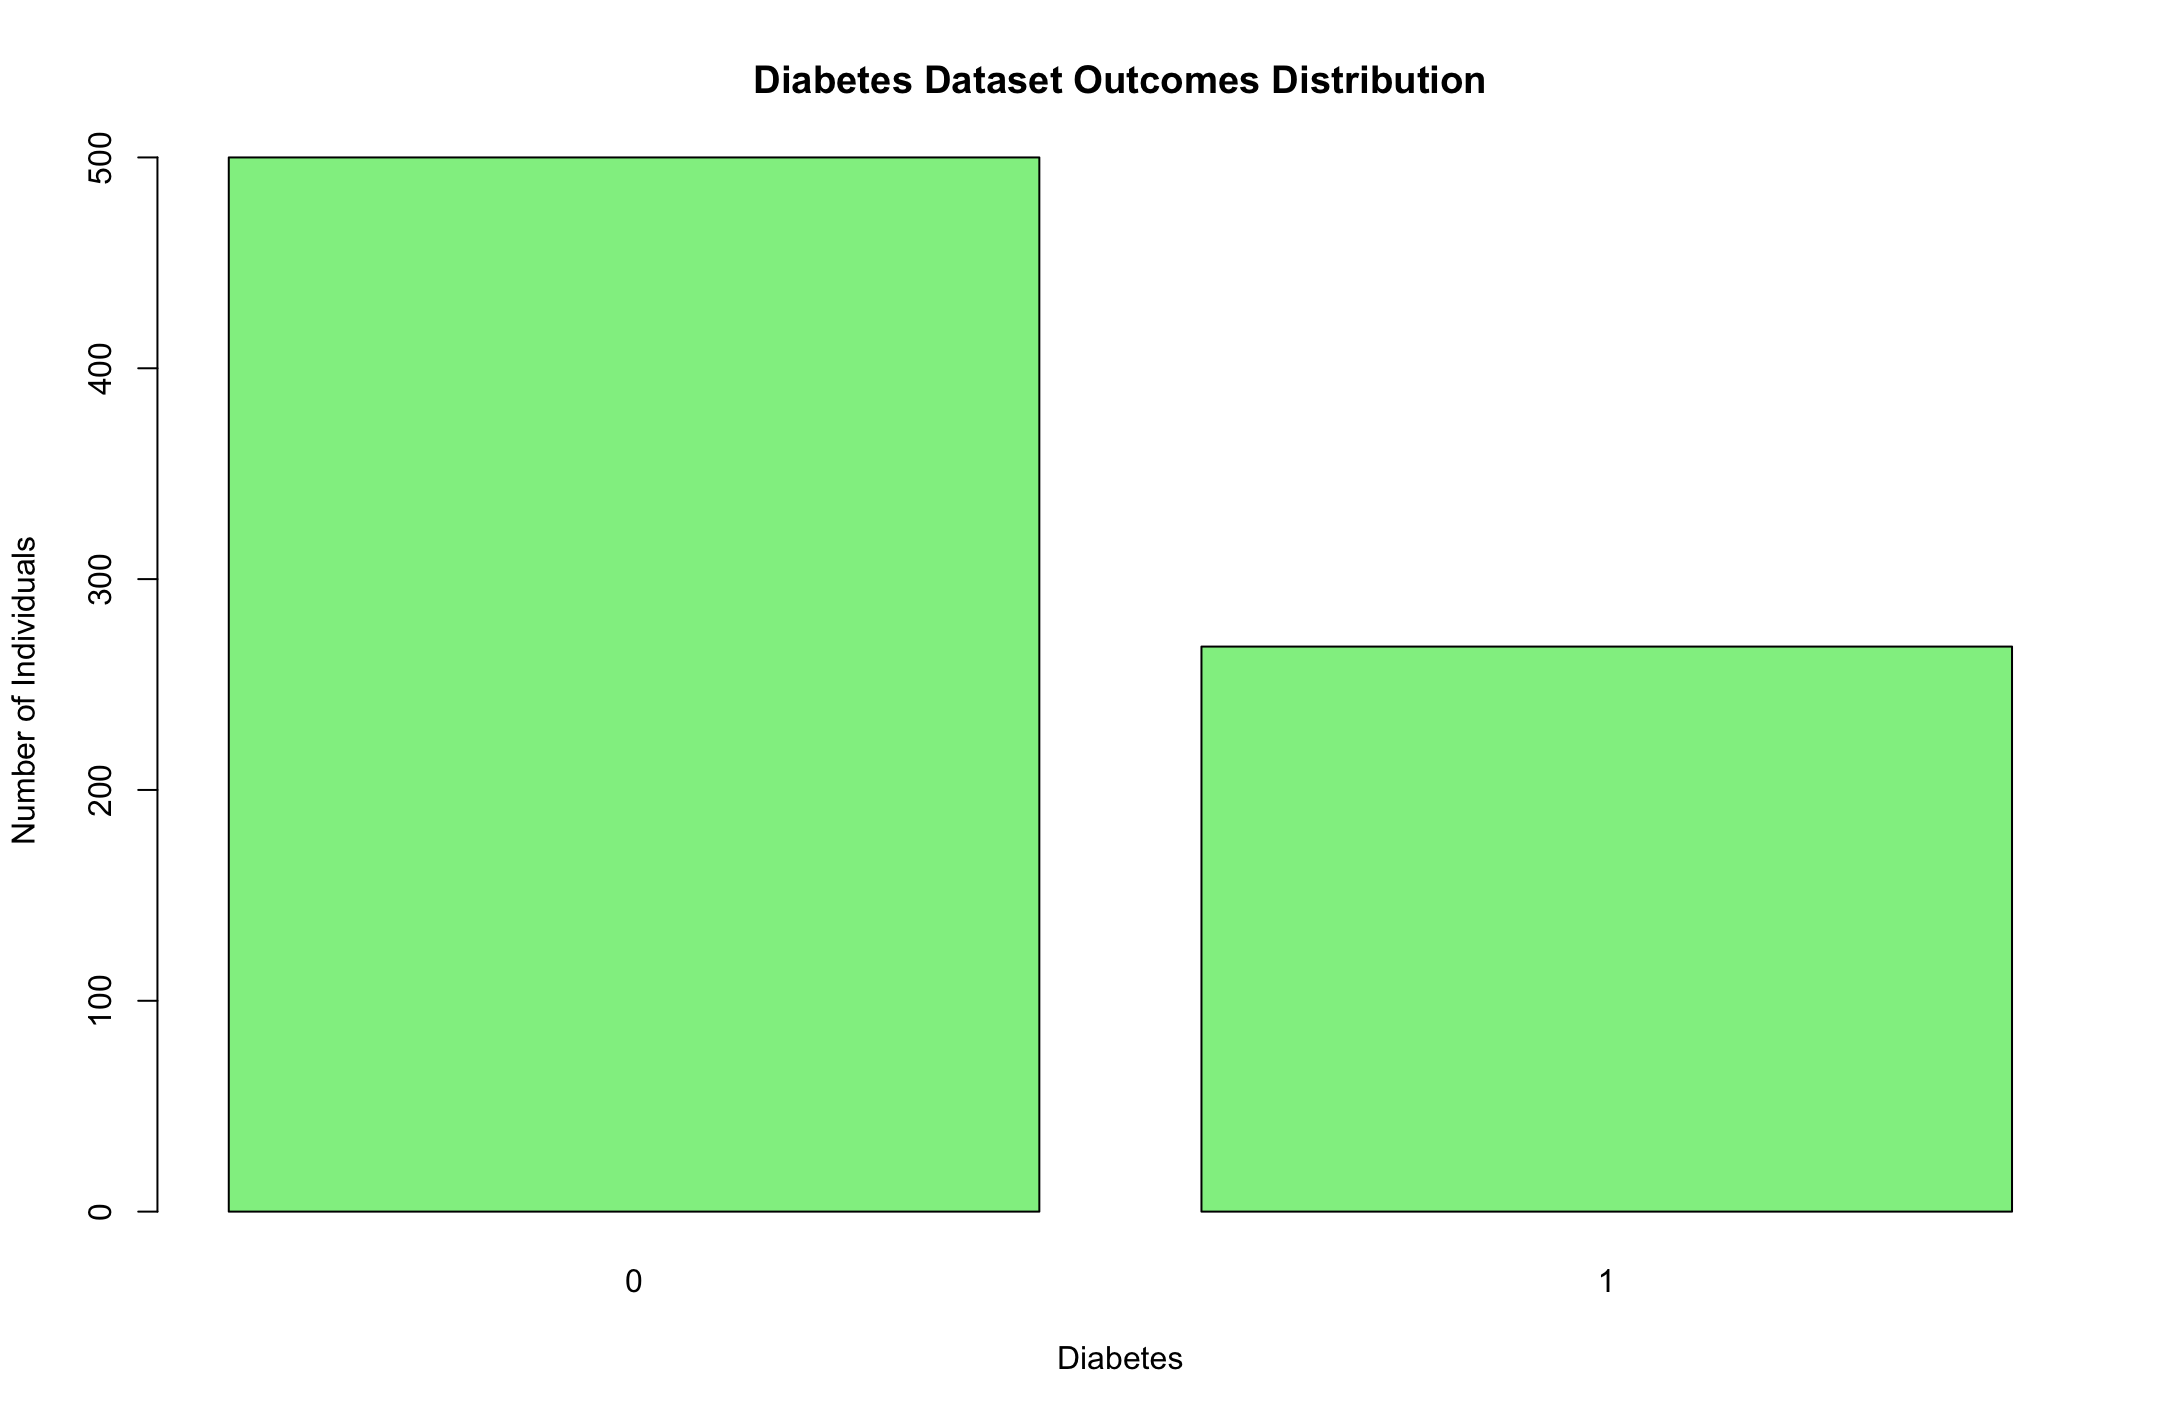
\includegraphics[width=\textwidth]{outcomes.png}} 
		\caption{Distribution of Outcomes} 
		\label{fig:outcomeplot}
	\end{minipage}
\end{figure}

\begin{figure}[h!]
	\centering
	% First figure
	\begin{minipage}{0.48\textwidth}
		\fbox{{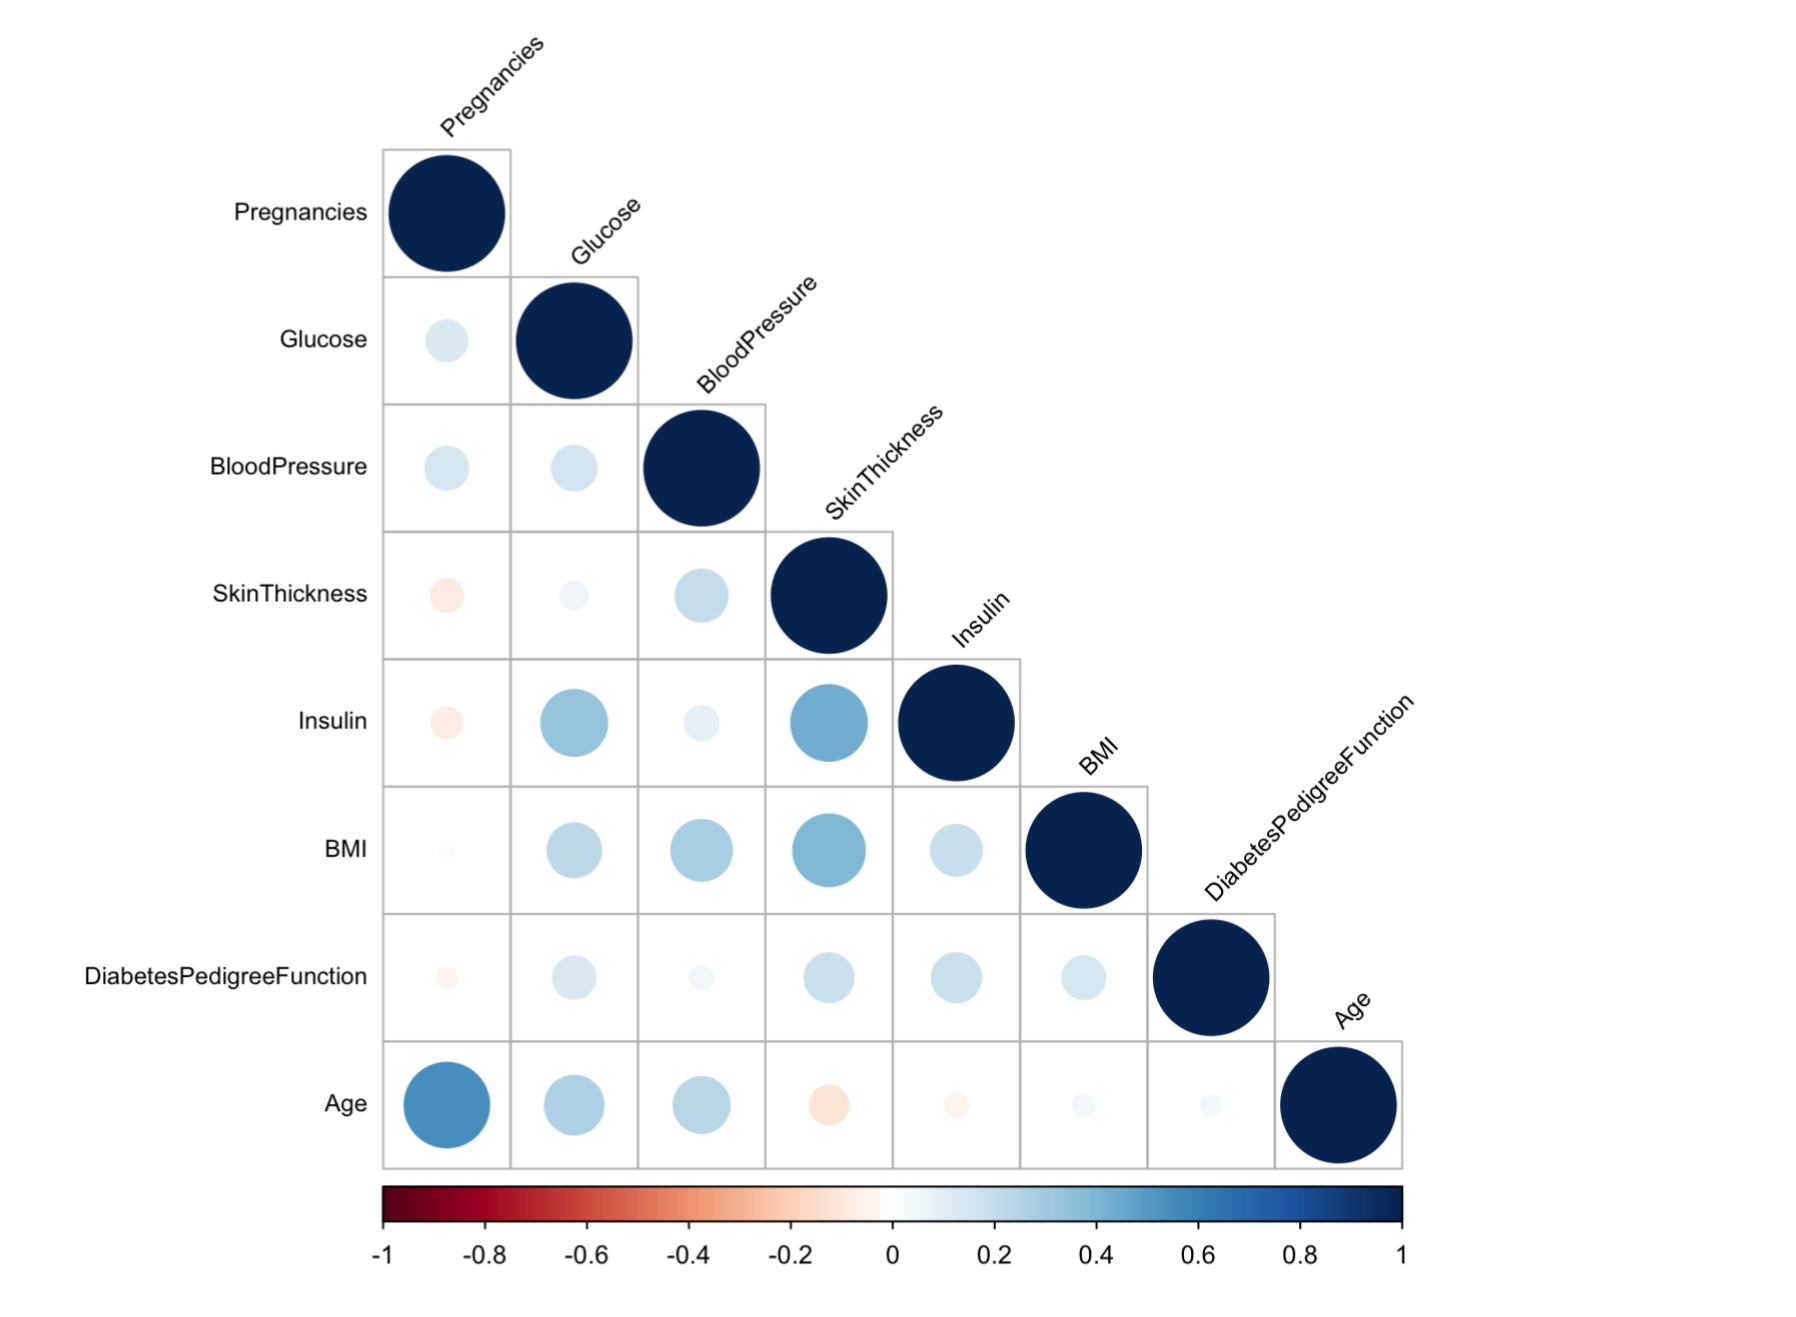
\includegraphics[width=\textwidth]{correlations2.png}}}
		\caption{Correlation of Variables} 
		\label{fig:corplot}
	\end{minipage}
	\hfill % Horizontal space between figures
	% Second figure
	\centering
	\begin{minipage}{0.48\textwidth}
		\centering
		\fbox{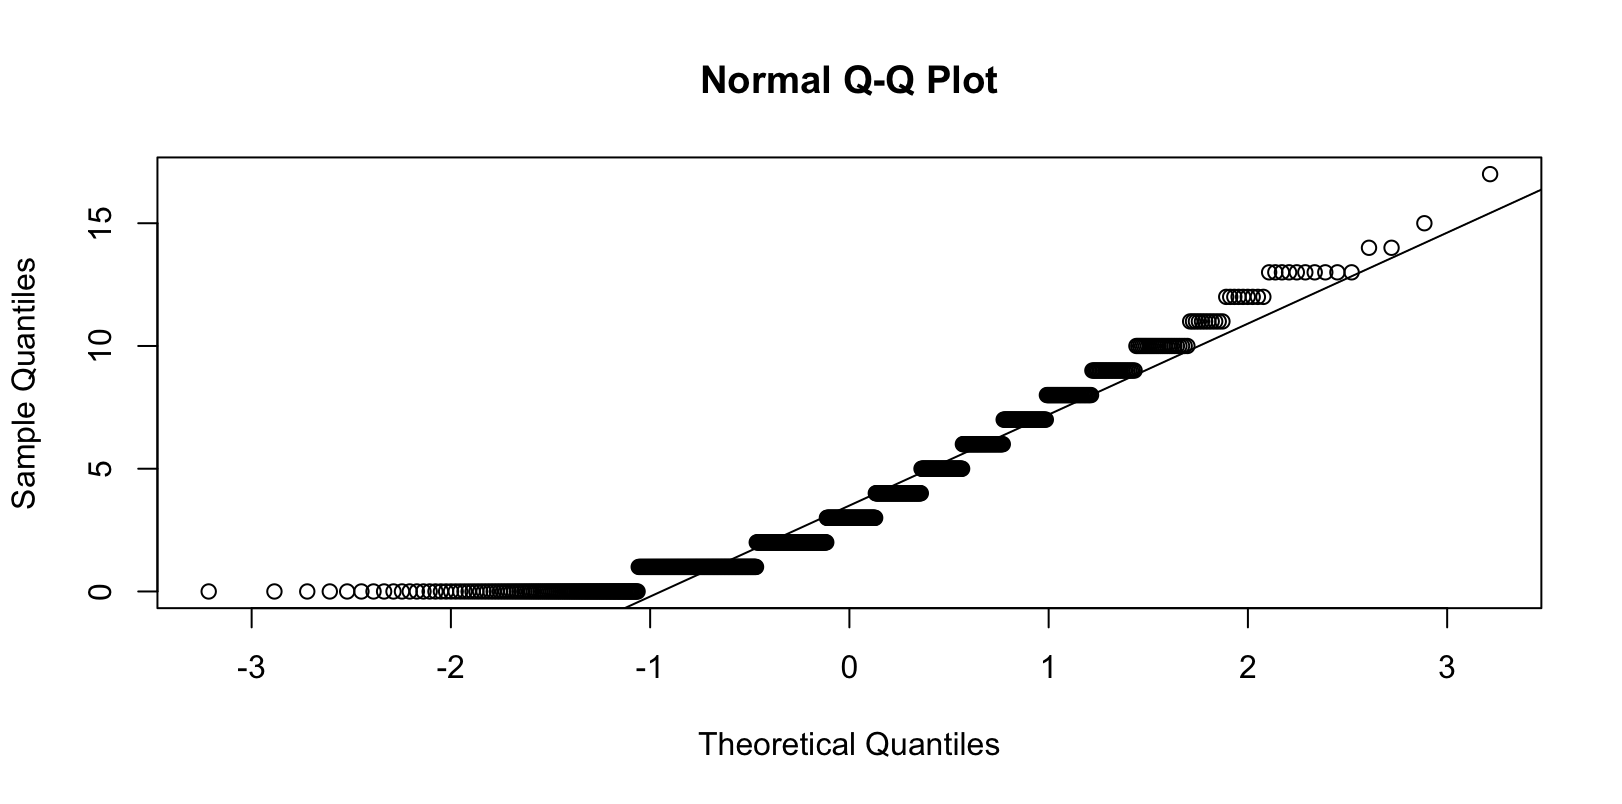
\includegraphics[width=\textwidth]{normal.png}} 
		\caption{Normal QQ-Plot} 
		\label{fig:qqplot}
	\end{minipage}
\end{figure}
		
\subsubsection{Data Preparation} 

We write about the training and testing here, and how we used column 9 as a label. We also scaled the dataset.\\

\section{Methodology}
\subsection{Supervised learning Analysis} 
 In this section, we perform supervised learning analysis using Classification trees: k-Nearest Neighbours and the following ensembles method: Random Forests Classifiers.\cite{zhou2012ensemble}
 
 \subsubsection{k-Nearest Neighbours}

 Firstly, we executed the k-Nearest Neighbours algorithm \cite{peterson2009k} on our dataset. The algorithm is a non-parametric, supervised learning classifier that uses proximity to make classifications about the grouping of a dataset.

 \subsubsection{Random Forest Classifiers}
 
 Also, we used the Random Forest Classifiers \cite{zhou2012ensemble} on our dataset. Random Forest classifiers is a bootstrapping sampling method that combines the results of multiple decision trees to draw on a conclusion. The algorithm \cite{Lecture16} is an extension of the bagging algorithm \cite{Lecture16} that creates uncorrelated decision trees, for each tree, a random sample of $\mathcal{M}$ is taken at each decision tree split.

\subsection{Binary Logistic Regression}

\begin{indent}
	

We performed binary logistic regression \cite{faraway2016extending} on our dataset to explore the relationship and significance between our predictor variables and the binary response variable “Outcome." The initial model uses all eight predictor variables.The objective of using binary logistic regression was to identify the most significant predictors using backward elimination, a step-wise technique employed in regression. This means that predictors whose $p$-value is greater than $\alpha = 0.05$ level of significance will be removed and we will run the algorithm again, repeating this process until we end up with only statistically significant predictors in our model --- minimizing the risk of over-fitting. 

\end{indent}

\subsection{Boosting}

Boosting \cite{chen2015xgboost} \cite{friedman2001greedy} is one of the ensembles methods which combines multiple weak learners, typically decision trees, to create a strong predictive model. For this analysis, we used XGBoost (Extreme Gradient Boosting), which is efficient and optimized for large datasets, to predict the presence of diabetes based on our predictor variables.

The model was trained on 75\% of the data, leaving 25\% for testing. The binary outcome variable (1 = diabetes, 0 = no diabetes) was predicted using features such as glucose levels, BMI, and age. Missing or zero values were present in some predictors (e.g., insulin), which could influence the model's performance.

\textbf{Model Parameters}
\begin{itemize}
	\item Learning rate (\texttt{eta}): 0.1
	\item Maximum tree depth (\texttt{max\_depth}): 6
	\item Evaluation metric: Area Under the Curve (AUC)
	\item Number of boosting rounds (\texttt{nrounds}): 100
\end{itemize}

\section{Discussion}
\subsection{Binary Logistic Regression}

\begin{table}[h!]
	\centering
	\resizebox{=0.9\textwidth}{!}{ % Resize to fit the width of the page
		\begin{tabular}{|c|c|c|c|c|}
			\hline
			\textbf{Coefficients} & \textbf{Estimate} & \textbf{Std. Error} & \textbf{Z-Value} & \textbf{Pr(>|Z|)} \\ \hline
			(Intercept) & -0.863576 & 0.111504 & -7.745 & 9.57E-15 \\ \hline
			Pregnancies & 0.411598 & 0.128257 & 3.209 & 1.33E-03 \\ \hline
			Glucose & 1.003291 & 0.133428 & 7.519 & 5.51E-14 \\ \hline
			BloodPressure & -0.15522 & 0.122145 & -1.271 & 0.2038 \\ \hline
			SkinThickness & -0.008376 & 0.123519 & -0.068 & 0.94594 \\ \hline
			Insulin & -0.160385 & 0.120504 & -1.331 & 1.83E-01 \\ \hline
			BMI & 0.699525 & 0.135793 & 5.151 & 2.59E-07 \\ \hline
			DiabetesPedigreeFunction & 0.295516 & 0.114215 & 2.587 & 0.00967 \\ \hline
			Age & 0.212147 & 0.127142 & 1.669 & 0.0952 \\ \hline
		\end{tabular}
	}
	\caption{Binary Logistic Regression Full Model Output}
	\label{tab:BinLogReg}
\end{table}

From (Table~\ref{tab:BinLogReg}), we see that the coefficients for “BloodPressure,” “SkinThickness,” “Insulin,” and "Age" have high p-values, indicating that at $\alpha = 0.05$ level of significance, they are not significant in predicting the "Outcome". At this step, the full binary logistic regression model outputs a Misclassification Rate (MCR) of  0.3697917.

\begin{table}[h!]
	\centering
	\resizebox{=0.90\textwidth}{!}{%
	\begin{tabular}{|c|c|c|c|c|}
		\hline
			\textbf{Coefficients:} & \textbf{Estimate} & \textbf{Std. Error} & \textbf{Z-Value} & \textbf{Pr(>|Z|)} \\ 
		\hline
		(Intercept)   & -7.90218 & 0.71505 & -11.051 & <2e-16 \\ 
		\hline
		Pregnancies   & 0.14734  & 0.03174 & 4.642   & 3.45E-06 \\ 
		\hline
		Glucose       & 0.03135  & 0.00375 & 8.359   & <2e-16 \\ 
		\hline
		BMI           & 0.08415  & 0.01597 & 5.269   & 1.37E-07 \\ 
		\hline
		DiabetesPedigreeFunction & 0.863621 & 0.336274 & 2.568 & 0.0102 \\ \hline
		Age & 0.029419 & 0.010701  & 2.749 & 0.00598 \\ \hline
	\end{tabular}%
	}
	\caption{Binary Logistic Regression Reduced Model Output}
	\label{tab:BinLogRegA}
\end{table}

Table~\ref{tab:BinLogRegA} contains the output from the Reduced Binary Logistic Regression Model. We observe that at $\alpha=0.05$ level of significance, every coefficient in the model is statistically significant in predicting diabetes Outcome. This is further reinforced given that the reduced model outputs an MCR of 0.2395833, i.e. $~76\%$ of individuals who were predicting to have, or not develop diabetes were correctly classified, indicating enhanced model performance. Consequently, we conclude that "Pregnancies," "Glucose," "BMI," and "DiabetesPedigreeFunction" all have a significant influence on the “Outcome”. This suggests a strong association between these factors and the risk of diabetes in females. \\


\subsection{Boosting}

The model achieved an accuracy of 80.5\% on the test set, with an AUC of 0.87. The AUC, derived from the ROC curve (Figure~\ref{fig:roc}), indicates that the model performs well in distinguishing between diabetic and non-diabetic individuals.

\begin{figure}[h!]
	\centering
	\fbox{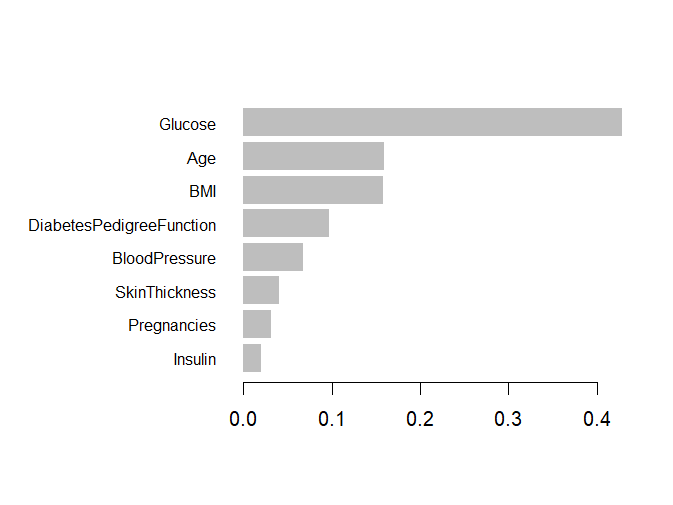
\includegraphics[width=0.7\textwidth]{"C:/Users/msafi/OneDrive/Documents/GitHub/4m_final_project/G1.png"}}
	\caption{ROC Curve for Boosting Model}
	\label{fig:roc}
\end{figure}

The feature importance plot (Figure~\ref{fig:importance}) reveals that glucose is the most significant predictor, followed by age, BMI, and genetic predisposition (DiabetesPedigreeFunction). These results align with established medical understanding of diabetes risk factors.

% \begin{figure}[h!]
% 	\centering
% 	% First figure
% 	\begin{minipage}{0.47\textwidth}
% 		\fbox{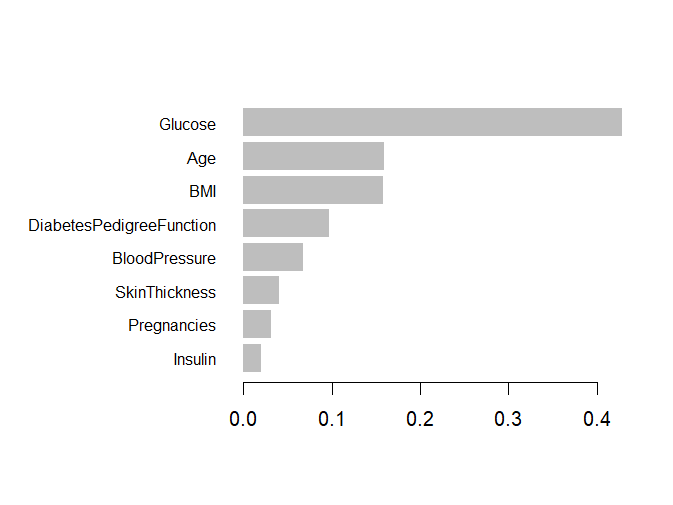
\includegraphics[width=\textwidth]{"C:/Users/msafi/OneDrive/Documents/GitHub/4m_final_project/G1.png"}}
% 		\caption{ROC Curve for Boosting Model}
% 		\label{fig:roc}
% 	\end{minipage}
% 	\hfill % Horizontal space between figures
% 	% Second figure
% 	\begin{minipage}{0.47\textwidth}
% 		\centering
% 		\fbox{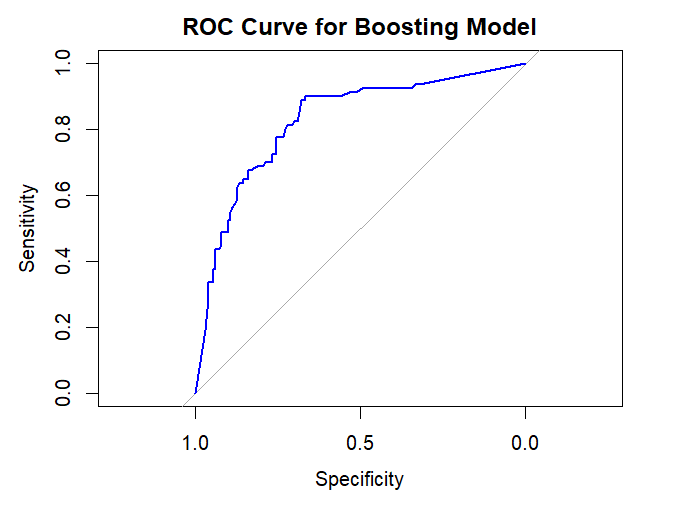
\includegraphics[width=\textwidth]{"C:/Users/msafi/OneDrive/Documents/GitHub/4m_final_project/G2.png"}}
% 		\caption{Feature Importance Plot}
% 		\label{fig:importance}
% 	\end{minipage}
% \end{figure}

\begin{figure}[h!]
	\centering
	\fbox{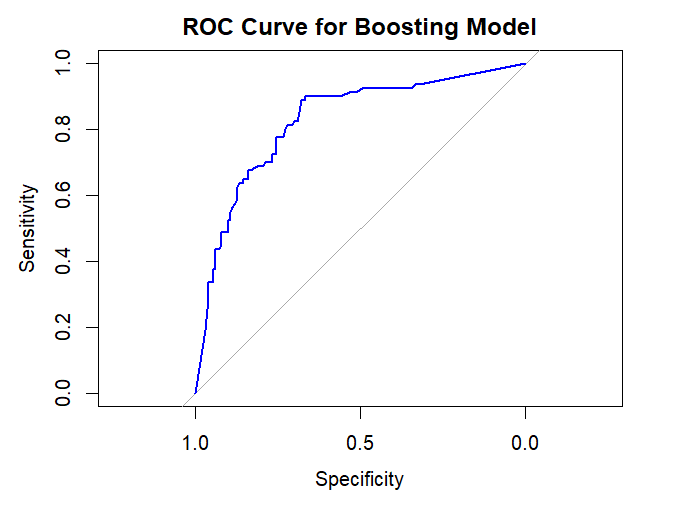
\includegraphics[width=0.7\textwidth]{"C:/Users/msafi/OneDrive/Documents/GitHub/4m_final_project/G2.png"}}
	\caption{Feature Importance Plot}
	\label{fig:importance}
\end{figure}


Boosting effectively identified significant predictors of diabetes, particularly glucose and BMI. However, the model's performance may be affected by missing data and the dataset's limited size. Future work could address these limitations by imputing missing values and validating the model on larger datasets. Overall, XGBoost proved to be a robust method for this binary classification problem.

\subsection{k-Nearest Neighbours}

% might want to include plot
After running tune.knn() with $5$-fold cross validation to get the parameters for the k-nearest neighbours algorithm (k-NN), we found that the best value for $k$ is $3$. After inputting $k=3$ and running the k-NN algorithm, we found that the MCR given by k-NN classification is $0.2916667$, i.e. $~71\%$ of the individuals with or without diabetes were correctly classified.

\begin{figure}[h!]
	\centering
	\fbox{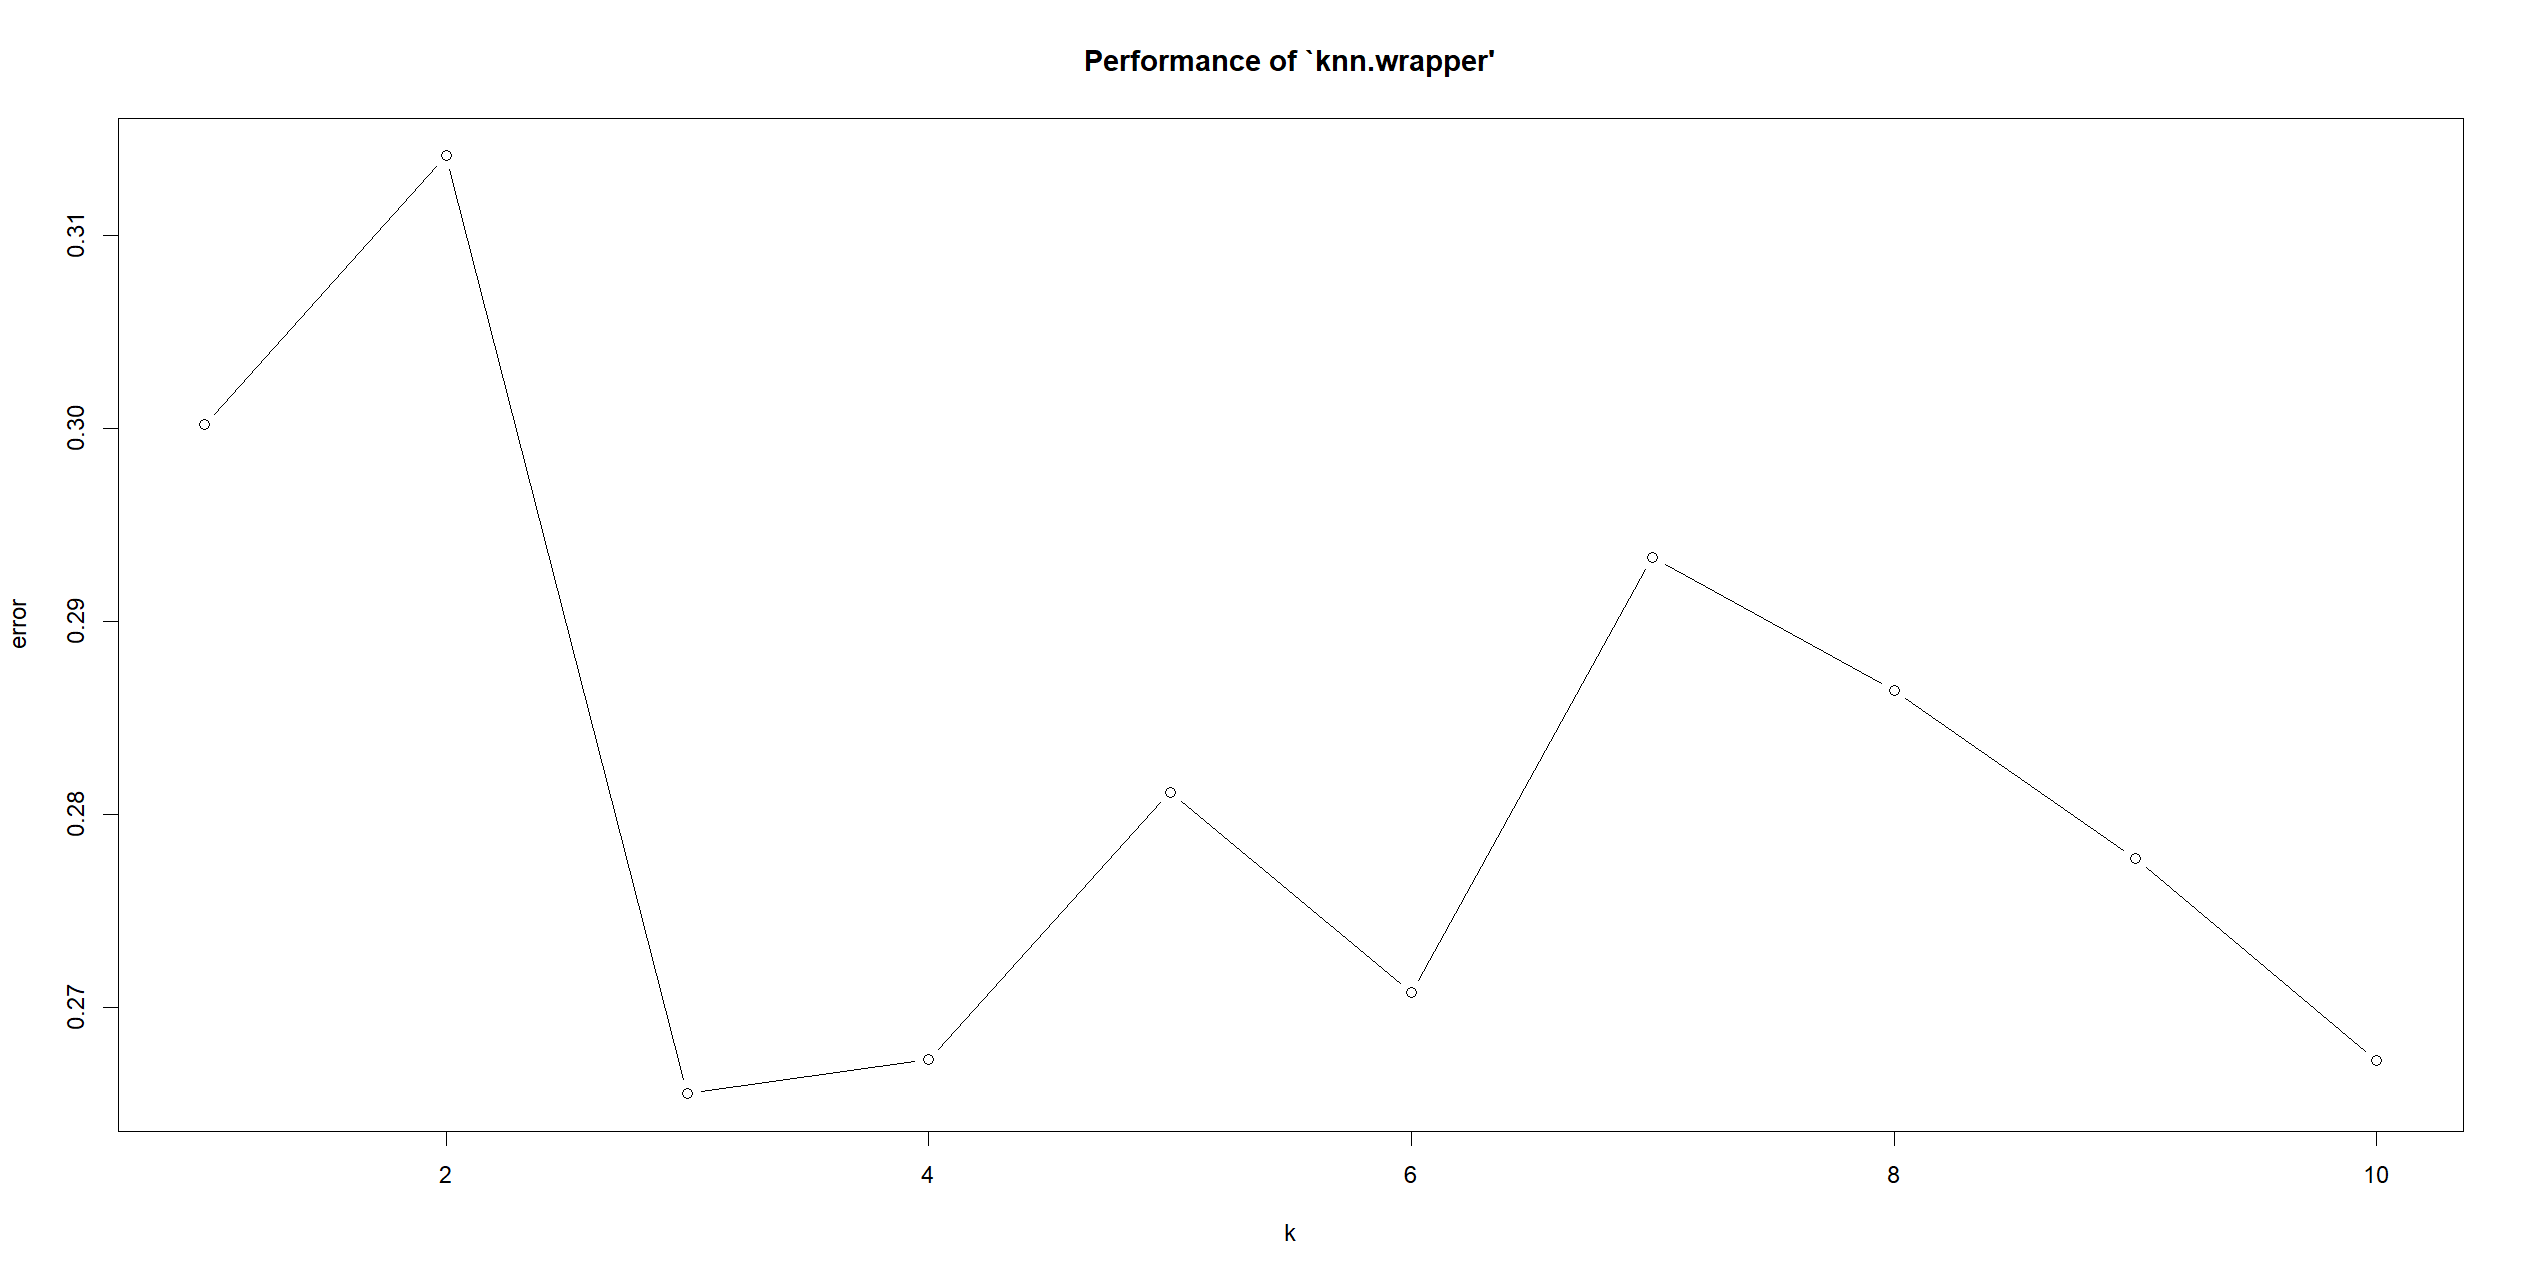
\includegraphics[width=0.7\textwidth]{knnplot.png}} 
	\caption{Output Plot From k-NN Classification} 
	\label{fig:KNNPlot}
\end{figure}

\subsection{Random Forest Classifiers}

%we wanna include the Variable importance plot here
After running tune.RandomForest() with $5$-fold cross validation to get the best parameters for the random forest algorithm, we found that the best value for $\mathcal{M}$ is $4$ and the best value of $M$ is $200$. 

After tuning and inputting $\mathcal{M}$ = $4$ and $M$ = $200$ into the random forest algorithm, we found that the MCR given by random forest classification is $0.28125$, i.e. $~72\%$ of the the individuals with or without diabetes were correctly classified.
Finally, we also observe that Glucose and BMI are the two most important variables according to the variable importance plot.

\begin{figure}[h!]
	\centering
	% First figure
	\fbox{{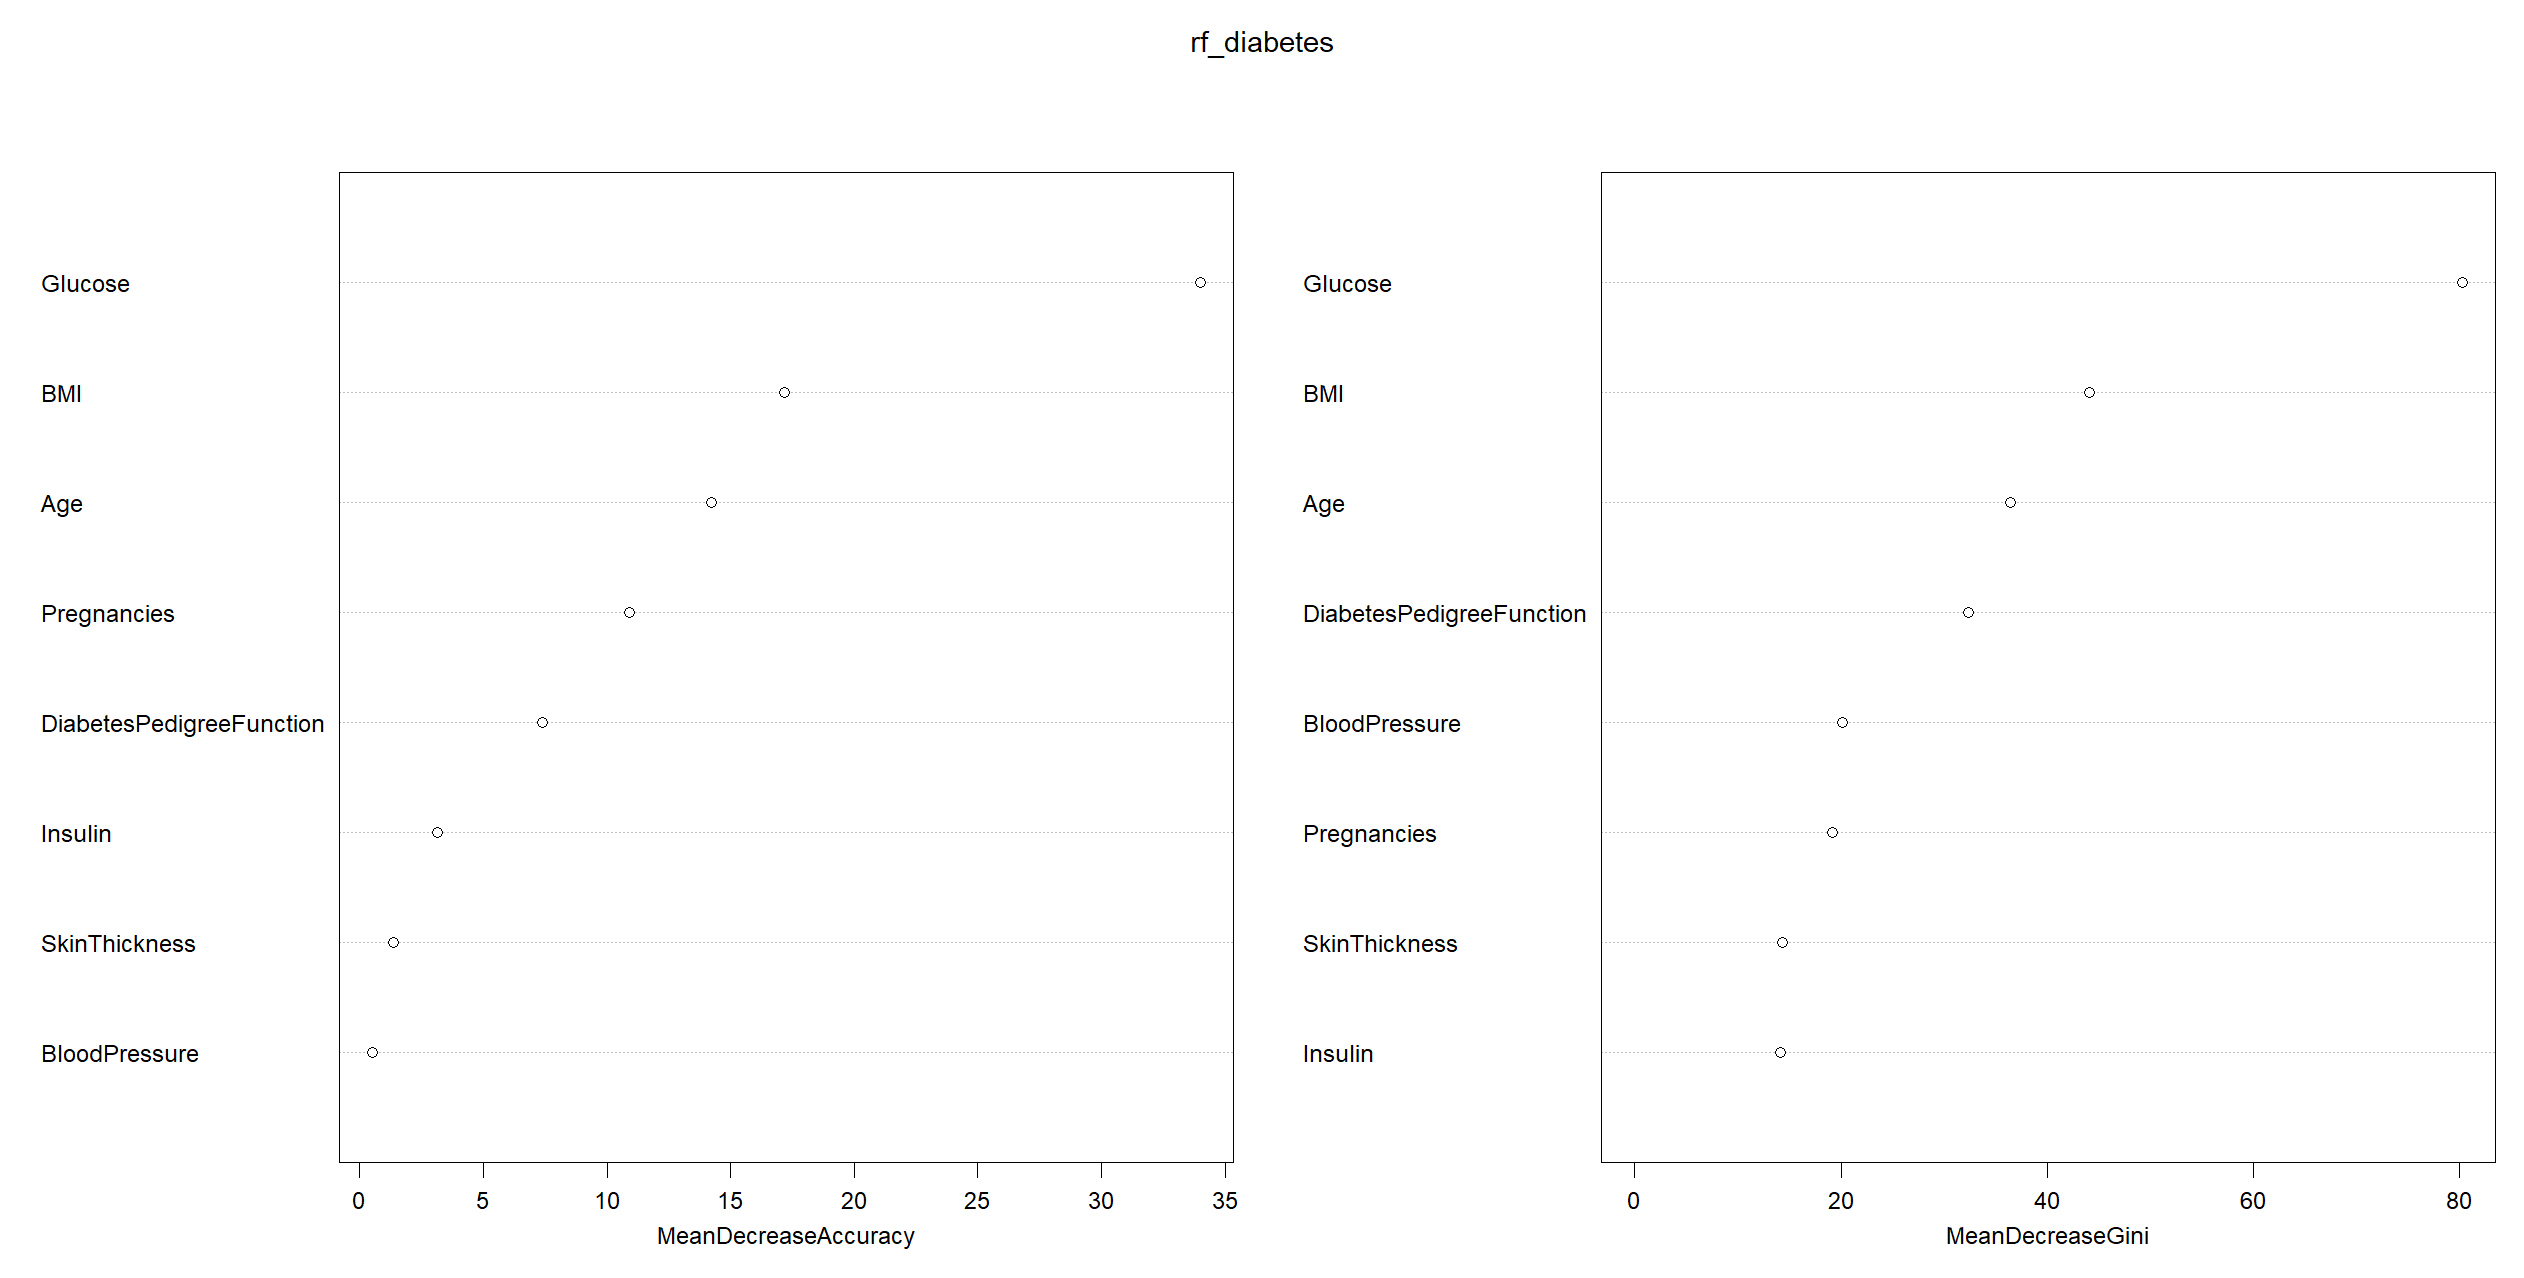
\includegraphics[width=0.7\textwidth]{MeanDecreaseAccuracyPlotForRandomForest.png}}}
	\caption{MeanDecreaseAccuracy Plot from Random Forest} 
	\label{fig:RFPlot}
\end{figure}


\section{Conclusion}

\textbf{TEMPORARY, WILL IMPROVE LATER} Comparison between supervised and unsupervised learning analysis, which method performs better for this dataset, which version of machine learning analysis helps us draw better conclusions for our dataset etc. 

 \section{Bibliography}
 \bibliographystyle{apa} 
 \bibliography{references}

\end{document}

